\section{Demostration Setup}
\label{sec:demo}
At the heart of our demonstration is a web-based ``Top-$k$'' list
extraction user interface \cite{list-extractor}.
It contains three main sections: TryItOut, Benchmark and Title. 
Under the TryItOut section, a user can test our system with an abitrary URL.
In the Benchmark section, we present 100 typical ``top-$k$'' pages
which the user can test either individually or in one go. We obtain
these benchmark pages by manually searching through over 5000 web pages
with ``top-$k$'' like titles.
And in the Title section, a user can test an abitrary page title 
(string) with the title classifier.

\begin{figure}[th]
	\centering
	\epsfig{file=./pic/Snapshot.eps,width=0.9\columnwidth}
\caption{Web Demo GUI: TryItOut}
\label{fig:gui}
\end{figure}

\begin{figure}[th]
	\centering
	\epsfig{file=./pic/benchmark1.eps,width=0.9\columnwidth}
\caption{Web Demo GUI: Benchmark}
\label{fig:gui2}
\end{figure}

\begin{figure}[th]
	\centering
	\epsfig{file=./pic/titleGUI2.eps,width=0.9\columnwidth}
\caption{Web Demo GUI: Title}
\label{fig:gui3}
\end{figure}

%Under Home tab, user can test any page by its URL, the system 
%will retrieve the page in real time 
%and attempt to extract a ``top-$k$'' list from it. 
%The output includes the page title, running time, number $k$, concepts 
%as well as the ``top-k list''.
%Under Benchmark tab, we provide a benchmark collection of 100 ``top-$k$'' pages. 
%Under Title tab, user can type a string as input, 
%and the system will analyze it as a page title and return detailed result.

A screenshot of the TryItOut section with blow-ups of extracted content
is shown in Figure \ref{fig:gui}.
Here, a user can type in the URL in the textbox and click ``Extract'' button, 
the system
will retrieve the page in real time and attempt to extract a ``top-$k$'' list from it. The output result includes
the page title, running time (in millisecond), number $k$, concepts as well as the ``top-$k$ list''. Both the
result and the original page will be presented after extraction.

In Benchmark section, as shown in Figure \ref{fig:gui2}, 
we list 100 ``top-$k$'' pages with their URLs. If a user want to test any one 
of them, she can click ``Test Me'' button, 
the browser will be redirected to TryItOut and show her the result. 
If the user wants to test the entire benchmark, she can click 
``Test All'' (in the bottom), the system will process
through the benchmark and send her a result file in XML format. 

In Title section, a user can type a string as input in
the textbox, then click ``Parse'' button, and the system will analyze it 
as a page title and return detailed result, including time, features, 
concepts and whether it is a ``top-$k$ like'' title.
A screenshot of this section is shown in Figure \ref{fig:gui3}.

\section{Conclusion}

%In this paper, we define a novel ``top-$k$'' list extraction problem 
%and give a solution with our system.
%Our evaluation shows that the system performs well in both accuracy and 
%efficiency, and able to scale to large web corpus and 
%obtain high-quality ``top-$k$'' lists,
%which is important in knowledge discovery and fact answering.

In this paper, we define a novel list extraction problem, 
which aims at recognizing, extracting
and understanding ``top-$k$'' lists from web pages. The problem is 
distinctive from other data mining tasks, because compared to other 
structured data, ``top-$k$'' lists are clearer, easier to understand and more
interesting for readers. Besides these advantages, 
``top-$k$'' lists are of great importance in knowledge discovery and 
fact answering simply because there are millions of ``top-$k$'' lists 
around on the web.
With the massive knowledge stored in those lists, we can enhance the 
instance space of a general purpose knowledge base such as Probase. 
It is also possible to build a search engine for ``top-$k$'' lists as 
an effective fact answering machine. Our proposed 4-stage 
extraction framework has demonstrated its ability to retrieve
large number of ``top-$k$'' lists at a very high precision.

%As a solution to this ``top-$k$'' problem, we present our system. The system mainly performs three
%tasks. First is to recognize ``top-k like'' title, which is done by the title classifier. In the classifier, we
%use a CRF-based model, trained from 6000 labeled titles, to identify whether a title is ``top-$k$ like''
%and obtain necessary information. Second is to extract ``top-$k$'' lists from the page body. To do this,
%we collect candidate lists based on tag path and the number $k$, and select the best one as the result. 
%Third is to further process the content of ``top-$k$'' lists, in which we infer the inner structure in the list content
%and split them into multiple fields.

